% !TEX encoding = UTF-8
% !TEX TS-program = pdflatex
% !TEX root = ../tesi.tex

%**************************************************************
\section{Sprint 6}
\label{sec:sprint6}
%**************************************************************

%**************************************************************
\subsection{User stories assegnate}
\paragraph{Raggruppamento dati (11)}\mbox{} \\[\baselineskip]
Come utente autenticato che si trova nella sezione “Reports”, voglio poter raggruppare i dati visualizzati per utente, cliente, progetto, task e data, con un massimo di 3 livelli di profondità.\\
Ad esempio, raggruppando per utente, la tabella mostrerà due colonne:
\begin{itemize}
  \item \texttt{Utente}, con i nomi di ogni utente;
  \item \texttt{Ore}, con la somma delle ore delle attività di ogni utente.
\end{itemize}
Se poi voglio aggiungere un secondo livello di profondità al raggruppamento, ad esempio per cliente, la tabella mostrerà sempre la colonna \texttt{Utente}, ma questa volta, sotto a ogni nome, saranno presenti delle ulteriori righe con i nomi dei vari clienti per cui l'utente ha svolto attività, con relative somme di ore.\\

\noindent Tasks:
\begin{itemize}
  \item implementare la funzionalità di raggruppamento;
  \item aggiungere la possibilità di raggruppamenti multipli;
  \item aggiungere una nuova sezione filtri dedicata ai raggruppamenti.
\end{itemize}

\paragraph{Esportazione report in formato CSV (3)}\mbox{} \\[\baselineskip]
Come utente autenticato che si trova nella sezione “Reports”, voglio poter esportare il report correntemente mostrato in un file CSV. 
Esso dovrà contenere tutti i dati mostrati nella tabella (anche eventuali dati presenti nelle pagine non correntemente mostrate).\\

\noindent Tasks:
\begin{itemize}
  \item aggiungere opzione per eseportare la tabella in formato CSV;
  \item aggiungere logica per la generazione del file CSV lato backend.
\end{itemize}


\subsection{Raggruppamento dati}
La prima cosa che ho fatto è stata la parte di frontend, aggiungendo 3 menù a tendina, uno per ogni livello di raggruppamento, da cui scegliere il campo da raggruppare. Il secondo e terzo menù sono inizialmente nascosti e compaiono solo quando rispettivamente il primo e secondo raggruppamento sono stati scelti.\\
Lato frontend ho aggiornato la richiesta principale al backend aggiungendo 3 parametri: \texttt{groupOne}, \texttt{groupTwo} e \texttt{groupThree}. Essi sono stringhe che di default assumono il valore \texttt{none} ma, nel caso sia selezionato un raggruppamento da parte dell'utente, assumono il nome di quel raggruppamento, ad esempio \texttt{project}.\\
Ho inoltre creato un altro component per le righe ``raggruppate'', in modo da ottenere una struttura tale che, se l'utente ha scelto due raggruppamenti, vengano inizialmente mostrate le righe del primo raggruppamento, potendo visualizzare quelle del secondo cliccando sulla rispettiva riga, come mostrato nella figura \ref{fig:report_groupedtable}.\\\\
\begin{figure}[H]
	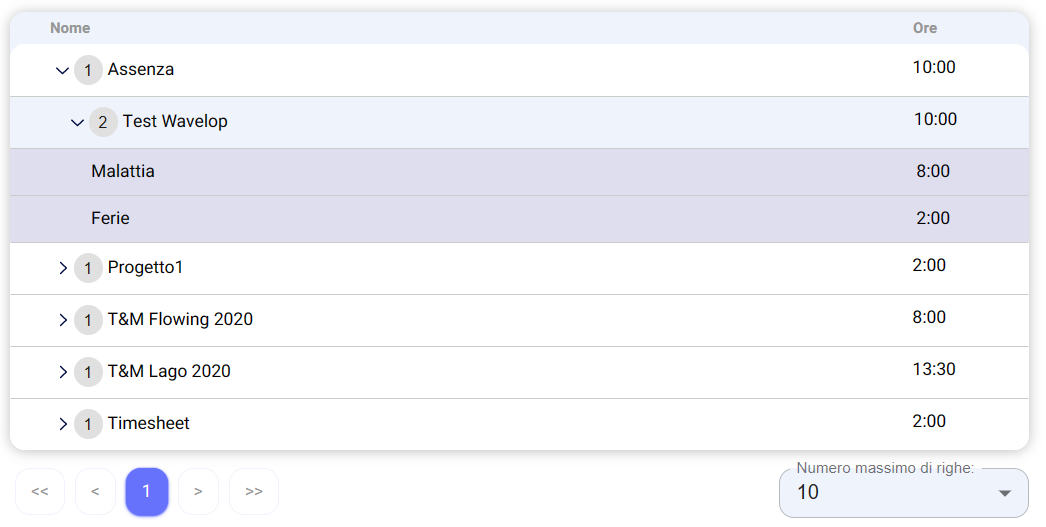
\includegraphics[width = \textwidth]{immagini/reports table groupings.png}
	\caption{Tabella che mostra dati raggruppati}
	\label{fig:report_groupedtable}
\end{figure}
Lato backend ho semplicemente aggiornato la query già presente in modo che potesse raggruppare i dati ottenuti, se richiesto. In questo caso i dati vengono ritornati con la seguente struttura:
\begin{itemize}
  \item \texttt{groupOne}
  \item \texttt{groupOneCount}
  \item \texttt{total}
\end{itemize}
Dove \texttt{groupOneCount} e \texttt{total} sono interi che rappresentano rispettivamente quanti elementi contiene il primo raggruppamento e la somma delle ore delle attività al suo interno.
\texttt{groupOne} è invece un array contenenti oggetti con la seguente struttura:
\begin{itemize}
  \item \texttt{name}: stringa contenente il nome della attività;
  \item \texttt{hours}: numero che rappresenta le ore dedicate all'attività;
  \item \texttt{groupTwo}: array contenente oggetti uguali a \texttt{groupOne}, eccetto relativi al secondo raggruppamento, più un campo \texttt{groupThree}.
\end{itemize}

\subsection{Esportazione report in formato CSV}
L'esportazione in formato CSV è risultata abbastanza rapida in quanto comportava solo ottenere i contenuti singoli dei campi richiesti dal frontend e porre tra di loro il carattere di separazione ``\texttt{,}''.\\
L'unica cosa a cui prestare attenzione è la eventuale presenza di virgole o virgolette nei campi che possano interferire col processo di separare i campi.
Per risolvere il problema basta circondare ogni campo tra virgolette.\\
Poi, tramite la funzione \texttt{join()}, ho unito tutti i campi di una riga ponendo fra loro il carattere \texttt{,} e separato le righe con il carattere di a capo \texttt{\textbackslash n}.\\
Lato frontend ho poi aggiunto un bottone che permette di scaricare il file CSV così creato.

\subsection{Sprint review}
La sprint review si è conclusa in modo positivo, ma è emerso un piccolo bug nella selezione dei raggruppamenti: selezionando primo, secondo e terzo raggruppamento e poi togliendo il secondo o il primo, il terzo raggruppamento rimaneva selezionato. La sistemazione di questo bug è rimasta assegnata per lo sprint 7.